% !Rnw weave = Sweave
\documentclass[xcolor={table}]{beamer}


\RequirePackage{../assets/pres-template_MOW}
\usepackage{colortbl}

%--------------------------------------------------------------------------
% Specific to this document ---------------------------------------


%--------------------------------------------------------------------------
% \setbeamercovered{transparent}

%%%%%%%%%%%%%%%%%%%%%%%%%%%%%%%%%%%
\setlength{\tabcolsep}{1.3pt}
\title{PLSC 40601}
\subtitle{Week 3: Trees and forests.}
\date{Spring 2024}
\author{Molly Offer-Westort}
\institute{Department of Political Science, \\University of Chicago}


\usepackage{Sweave}
\begin{document}
\input{plsc40601_slides_31-concordance}



%-------------------------------------------------------------------------------%
\frame{\titlepage
\thispagestyle{empty}
}
%-------------------------------------------------------------------------------%
\begin{frame}{Housekeeping}

\begin{wideitemize}
\item ?
\end{wideitemize}

\end{frame}


%%%%%NOTE%%%%%
\note{
\scriptsize \singlespacing

\begin{wideitemize}
\item xxxx
\end{wideitemize}

}

%-------------------------------------------------------------------------------%
\begin{transitionframe}
\centering

\LARGE \textcolor{white}{Trees}

\end{transitionframe}
%-------------------------------------------------------------------------------%
\begin{frame}{Regression Trees}

\begin{wideitemize}
\item Suppose we have joint data, $(Y,X_1, X_2)$.\pause
\item Our goal is to partition the data with the objective of prediction. 
\end{wideitemize}

\begin{figure}
\centering
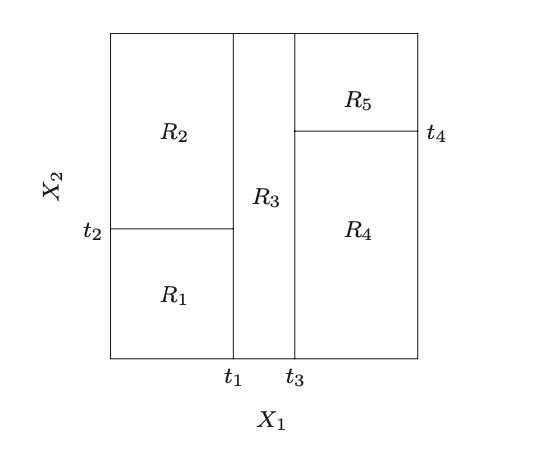
\includegraphics[width = 0.6\textwidth]{../assets/tibshirani9-1.png}
\end{figure}
\hfill \cite{hastie2009elements}


\end{frame}


%%%%%NOTE%%%%%
\note{
\scriptsize \singlespacing

\begin{wideitemize}
\item xxxx
\end{wideitemize}
\\~\
}

%-------------------------------------------------------------------------------%

\begin{frame}{Regression Trees}

\begin{wideitemize}
\item Our model is
\[
f(\X) = \sum_{m = 1}^M c_m \mathbbm{1}\{\X\in R_m\}
\]\pause
\item Our objective is
\[
\sum_{i = 1}^N\left(y_i - \hat{f}(\x_i)\right)^2
\]\pause
\item With fixed regions $R_m$, how should we pick $\hat c_m$?\pause
\[
\hat c_m=   \bar y_{\x_{i}\in R_m}
 \]
\end{wideitemize}


\end{frame}


%%%%%NOTE%%%%%
\note{
\scriptsize \singlespacing

\begin{wideitemize}
\item xxxx
\end{wideitemize}
\\~\
}

%-------------------------------------------------------------------------------%

\begin{frame}{Regression Trees}

\begin{wideitemize}
\item How do we pick partitions?\pause
\item A greedy approach:\pause
\begin{wideitemize}
\item splitting var $j$, split point $s$, 
\[
R_1(j,s) = \{ X|X_j \le s\} \textrm{ and } R_1(j,s) = \{ X|X_j > s\}
\]
\pause
\item Solve
\[
\underset{j,s}{\textrm{min}}\left[\underset{c_1}{\textrm{min}} \sum_{i:x_{j[i]} \in R_1(j,s)}(y_i -c_1)^2 + \underset{c_2}{\textrm{min}} \sum_{i:x_{j[i]} \in R_2(j,s)}(y_i -c_2)^2 \right]
\]\pause
\item The inner minimization problem is again solved by averages. 
\[
\hat c_1= \bar y_{x_{j[i]}\in R_1(j,x)} \textrm{ and } \hat c_2=  \bar y_{x_{j[i]}\in R_2(j,x)}
 \]\pause
 \item Then pick $s$ to solve the outer minimization problem for a given variable $j$. 
\end{wideitemize}
\end{wideitemize}


\end{frame}


%%%%%NOTE%%%%%
\note{
\scriptsize \singlespacing

\begin{wideitemize}
\item xxxx
\end{wideitemize}
\\~\
}

%-------------------------------------------------------------------------------%

\begin{frame}{Regression Trees}

\begin{wideitemize}
\item For just one variable:
\end{wideitemize}


\end{frame}


%%%%%NOTE%%%%%
\note{
\scriptsize \singlespacing

\begin{wideitemize}
\item xxxx
\end{wideitemize}
\\~\
}

%-------------------------------------------------------------------------------%
\begin{frame}[fragile]

\begin{figure}
\centering
{
\includegraphics{plsc40601_slides_31-002}
}
\end{figure}

\end{frame}


%%%%%NOTE%%%%%
\note{
\scriptsize \singlespacing

\begin{itemize}
\item xxxx
\end{itemize}
\\~\
}

%-------------------------------------------------------------------------------%
\begin{frame}[fragile]

\begin{figure}
\centering
{
\includegraphics{plsc40601_slides_31-003}
}
\end{figure}

\end{frame}


%%%%%NOTE%%%%%
\note{
\scriptsize \singlespacing

\begin{itemize}
\item xxxx
\end{itemize}
\\~\
}

%-------------------------------------------------------------------------------%
\begin{frame}{Regression Trees}

\begin{itemize}
\item Now suppose we have joint data, $(Y,X_1, \dots, X_k)$.\pause
\item We will do the same approach to finding thresholds to minimize prediction error, but we'll want to pick which $X_k$ we use for threshholding, as well. \pause
\item Generally, we'll define the depth of the tree as 2 or three variables; first we'll split on $X_k$, then we'll split on $X_j$\dots
\end{itemize}


\end{frame}


%%%%%NOTE%%%%%
\note{
\scriptsize \singlespacing

\begin{itemize}
\item xxxx
\end{itemize}
\\~\
}
%-------------------------------------------------------------------------------%
\begin{frame}[fragile]{Elements of trees}

\begin{Schunk}
\begin{Sinput}
> n <- 500
> p <- 10
> X <- matrix(rnorm(n * p), n, p)
> W <- rbinom(n, 1, 0.5)
> Y <- pmax(X[, 1], 0) * W + X[, 2] +
+   pmin(X[, 3], 0) + rnorm(n)
> c.forest <- causal_forest(X, Y, W)
> tree <- get_tree(c.forest, 1)
> leaf.nodes <- get_leaf_node(tree, X[1:5, ])
\end{Sinput}
\end{Schunk}



\end{frame}


%%%%%NOTE%%%%%
\note{
\scriptsize \singlespacing

\begin{wideitemize}
\item xxxx
\end{wideitemize}

}

%-------------------------------------------------------------------------------%
\begin{frame}[fragile]{Elements of trees}
\small
\begin{Schunk}
\begin{Sinput}
> tree
\end{Sinput}
\begin{Soutput}
GRF tree object 
Number of training samples: 250 
Variable splits: 
(1) split_variable: X.5  split_value: -0.520294 
  (2) split_variable: X.4  split_value: 0.426613 
    (4) split_variable: X.9  split_value: -0.314623 
      (8) * num_samples: 7  avg_Y: 0.09 avg_W: 1 
      (9) * num_samples: 14  avg_Y: 0.11 avg_W: 0.43 
    (5) * num_samples: 8  avg_Y: -0.49 avg_W: 0.38 
  (3) split_variable: X.2  split_value: -0.344787 
    (6) split_variable: X.6  split_value: 0.163222 
      (10) * num_samples: 23  avg_Y: -0.9 avg_W: 0.48 
      (11) * num_samples: 11  avg_Y: -1.87 avg_W: 0.82 
    (7) split_variable: X.3  split_value: 0.428785 
      (12) split_variable: X.3  split_value: -0.322743 
        (14) * num_samples: 18  avg_Y: -0.29 avg_W: 0.61 
        (15) * num_samples: 14  avg_Y: 0.64 avg_W: 0.5 
      (13) * num_samples: 30  avg_Y: 0.72 avg_W: 0.47 
\end{Soutput}
\end{Schunk}


\end{frame}


%%%%%NOTE%%%%%
\note{
\scriptsize \singlespacing

\begin{wideitemize}
\item xxxx
\end{wideitemize}

}

%-------------------------------------------------------------------------------%
\begin{frame}{A tree}

\begin{figure}
\centering
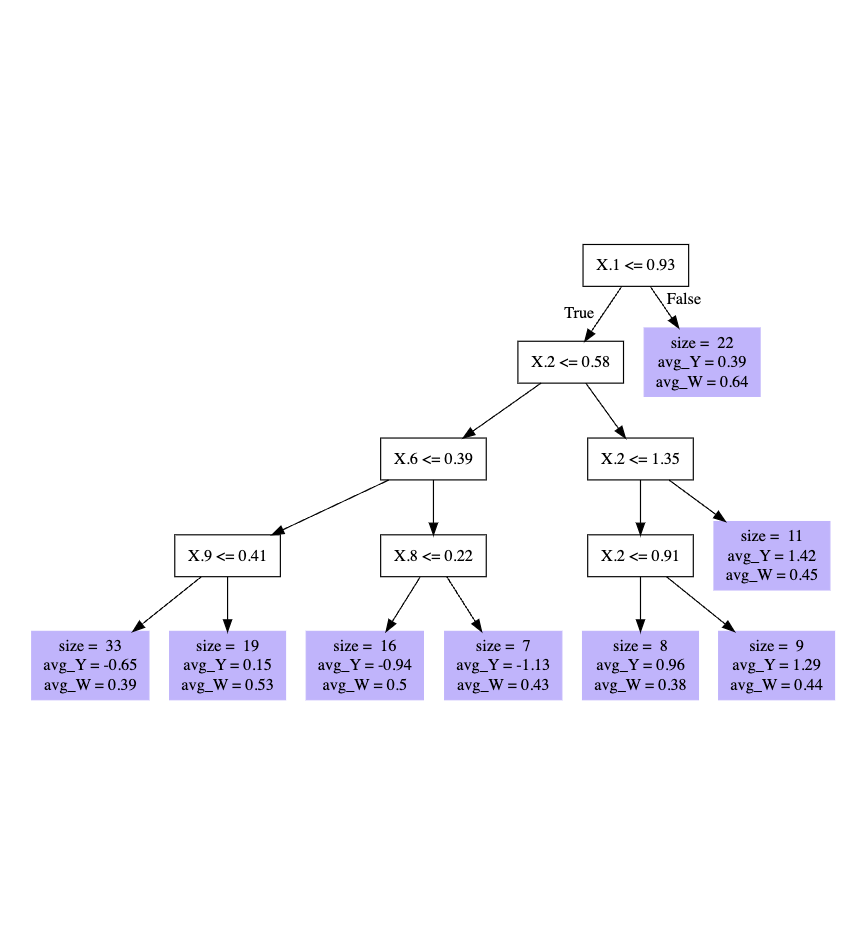
\includegraphics[width = 0.8\textwidth]{../assets/tree-plot.png}
\end{figure}
\hfill
\end{frame}


%%%%%NOTE%%%%%
\note{
\scriptsize \singlespacing

\begin{wideitemize}
\item xxxx
\end{wideitemize}

}

%-------------------------------------------------------------------------------%

\begin{frame}{Elements of trees}


\begin{wideitemize}
\item Node\pause
\item Split/branches\pause
\item Leaves
\end{wideitemize}

\end{frame}


%%%%%NOTE%%%%%
\note{
\scriptsize \singlespacing

\begin{wideitemize}
\item xxxx
\end{wideitemize}

}

%-------------------------------------------------------------------------------%
\begin{frame}{Trees for classification}

\begin{wideitemize}
\item What about when $Y$ is a category? \pause
\item For binary classification, minimize surrogate for classification error with split point $s$, $I(s) = \sum_{t = 1}^2 \gamma_t$
\[
\gamma_t = 1 - \left[\bar Y^2_t + (1-\bar Y_t)^2  \right]
\]\pause
\item $I(s)$ measures the impurity of a partition. \pause What happens if $R_m$ has only 1's, or only 0s?
\pause
\item For multi-class classification, use Gini impurity, which generalizes using $\hat p_t(k)$, the proportion of class $k$ in partition $t$.\pause
\item Why impurity instead of classification error? \pause Smooth function, easier to minimize. \pause But there are other metrics we could use. \pause
\item We can extend these methods to more complex classification tasks. 
\end{wideitemize}


\end{frame}


%%%%%NOTE%%%%%
\note{
\scriptsize \singlespacing

\begin{wideitemize}
\item xxxx
\end{wideitemize}
\\~\
}

%-------------------------------------------------------------------------------%
\begin{frame}{Policy trees, or decision trees}


\begin{wideitemize}
\item Policy trees solve:
\end{wideitemize}
\[
\pi^{*} = \underset{\pi \in \Pi}{\textrm{argmax}} \left[ \frac{1}{N}\sum_{i = 1}^N \Gamma_i \left(\pi(X_i) \right) \right]
\]
\pause
\begin{align*}
    \Gamma_i&  =
     \frac 1 N  \sum_{i=1}^N \textcolor{Contrast1}{\underbrace{\hat{\E}[Y_i | W_i = w, X_i]}_\text{estimated outcome model}}+\\ 
     & \qquad \qquad \frac{1}{N} \sum_{i=1}^N  \underbrace{\frac{ \mathbbm{1} \{W_i = w \} \left( Y_i - \textcolor{Contrast1}{\hat{\E}[Y_i | W_i = w, X_i]} \right) }{ \textcolor{Contrast4}{ e_i(w;s)} }}_\text{residual bias correction}
\end{align*}


\end{frame}


%%%%%NOTE%%%%%
\note{
\scriptsize \singlespacing

\begin{wideitemize}
\item xxxx
\end{wideitemize}

}

%-------------------------------------------------------------------------------%
\begin{frame}{[Recall]}

\begin{wideitemize}
\item Estimating average treatment effects. \\ 
\begin{align*}
\mu(w,x) & = \E[Y_i |W_i = w, \X_i = x]\\
e(x) & = \E[W_i | \X_i = x]
\end{align*}
\begin{align*}
    \onslide<1->{\tau &= \E\left[\mu(1,\X_i) - \mu(0,\X_i) \right] \\}
    \onslide<1->{ & = \E\left[\frac{Y_i W_i}{e(\X_i)} - \frac{Y_i (1-W_i) }{1 - e(\X_i)}\right] \\}
    \onslide<1>{ & = \E\left[ \frac{\left(Y_i - \mu(1,\X_i)\right)  W_i}{e(\X_i)} - \frac{\left(Y_i - \mu(0,\X_i)\right) (1-W_i) }{1 - e(\X_i)}\right] \\}
   \onslide<1>{ & \qquad \qquad  + \E\left[\mu(1,\X_i) - \mu(0,\X_i) \right]}
\end{align*}
\end{wideitemize}

\end{frame}


%%%%%NOTE%%%%%
\note{
\scriptsize \singlespacing

\begin{wideitemize}
\item xxxx
\end{wideitemize}

}

%-------------------------------------------------------------------------------%

\begin{frame}{Tuning parameters}

\begin{wideitemize}
\item How do we pick which splitting variables to use?\pause
\item How many splits to complete? \pause
\item Pruning?
% \begin{wideitemize}
% \item Cost-complexity pruning: keep going until you get a fixed minimum node size. 
% \end{wideitemize}
\end{wideitemize}


\end{frame}


%%%%%NOTE%%%%%
\note{
\scriptsize \singlespacing

\begin{wideitemize}
\item xxxx
\end{wideitemize}
\\~\
}

%-------------------------------------------------------------------------------%
\begin{transitionframe}
\centering

\LARGE \textcolor{white}{Forests}

\end{transitionframe}

%-------------------------------------------------------------------------------%
\begin{frame}{Random forests\dots}
\pause

\begin{wideitemize}
\item Define a tree predictor or classifier as $h(\x, \Theta_k)$\pause
\item ${\Theta_k}$ are i.i.d. random vectors \pause (putting the \textit{random} in random forests)\pause
\item With predictors or classifiers $\{h(\x, \Theta_k), \ k = 1, \dots, K \}$, combine across trees, where estimates produced from each tree are averaged for prediction problems, and treated as votes for classification problems. 
\end{wideitemize}

\end{frame}


%%%%%NOTE%%%%%
\note{
\scriptsize \singlespacing

\begin{wideitemize}
\item xxxx
\end{wideitemize}

}

%-------------------------------------------------------------------------------%
\begin{frame}{Random forests\dots}

\begin{wideitemize}
\item Different types of forests use different approaches to random vectors $\Theta_k$. \pause
\item How to compare them?
\end{wideitemize}

\end{frame}


%%%%%NOTE%%%%%
\note{
\scriptsize \singlespacing

\begin{wideitemize}
\item xxxx
\end{wideitemize}

}

%-------------------------------------------------------------------------------%
\begin{frame}{Generalization error for forests}

For numerical predictors:
\[
PE^{*}_{\textrm{forest}} = \E_{\X,Y}\left[\left(Y - \E_{\Theta}\left[ h(\X, \Theta)\right]\right)^2\right]
\]\pause

\[
PE^{*}_{\textrm{tree}} = \E_{\Theta}\left[ \E_{\X,Y}\left[\left(Y - h(\X, \Theta)\right)^2\right]\right]
\]
\pause

\[
PE^{*}_{\textrm{forest}} \le \bar \rho PE^{*}_{\textrm{tree}}
\]
where $\bar \rho$ is a weighted correlation between $Y - h(\X, \Theta)$, $Y - h(\X, \Theta')$ where $\Theta, \Theta'$ are independent. \pause


Implication: for good generalization error of a forest, we need low correlation error across $\Theta$, and low error trees. 

\end{frame}


%%%%%NOTE%%%%%
\note{
\scriptsize \singlespacing

\begin{wideitemize}
\item xxxx
\end{wideitemize}

}

%-------------------------------------------------------------------------------%
\begin{frame}{Some approaches to forests}

\begin{wideitemize}
\item Adaptive reweighting of the training set (arcing), see Adaboost (\textcolor{Contrast4}{\textbf{ada}}ptive + \textcolor{Contrast4}{\textbf{boost}}ing) \citep{freund1996experiments} \pause (\textit{not} random)\pause
\item Bagging \pause
\item Forest RI: Random input selection at each node. \pause Don't prune. \pause Fix number of features used. \pause
\begin{itemize}
\item Tuning parameter: number of features used. \pause
\item Performs pretty well, even when number of features is small (1!)\pause
\item If total number of features is small, can result in high correlation. 
\end{itemize}\pause
\item Forest RC: Random combination of inputs selected at each node. \pause Fix number of features used, combine them with random coefficients. \pause Create a fixed number of combinations, and search over for the best.\pause
\begin{itemize}
\item Tuning parameters: number of features used, number of combinations of features. 
\end{itemize}
\end{wideitemize}

\end{frame}


%%%%%NOTE%%%%%
\note{
\scriptsize \singlespacing

\begin{wideitemize}
\item xxxx
\end{wideitemize}

}

%-------------------------------------------------------------------------------%
\begin{frame}{Some approaches to forests}

\begin{wideitemize}
\item Which approach works best depends on number of covariates, how correlated covariates are, how predictive covariates are. \pause
\item More (combinations of) features not always better. 
\end{wideitemize}

\end{frame}


%%%%%NOTE%%%%%
\note{
\scriptsize \singlespacing

\begin{wideitemize}
\item xxxx
\end{wideitemize}

}

%-------------------------------------------------------------------------------%
\begin{frame}{Other qualities}

In addition to low correlation across prediction error, and strength of trees, we might want methods that are\pause
\begin{wideitemize}
\item Robust to outliers\pause
\item Have good computational speed\pause
\item Have good internal metrics of error, strength, correlation, variable importance \pause
\item Possible to parallelize?
\end{wideitemize}

\end{frame}


%%%%%NOTE%%%%%
\note{
\scriptsize \singlespacing

\begin{wideitemize}
\item xxxx
\end{wideitemize}

}

%-------------------------------------------------------------------------------%
\begin{frame}{Internal metrics}

``Out-of-bag'' estimation \pause (we've seen this before)\pause
\[
 \hat f_i^{oob} = \frac{1}{\lvert C^{-i} \rvert}\sum_{b \in C^{-i}}\hat f^b (x_i)
\]
$C^{-i}$ is the set of bootstrap samples that do not contain $i$, $\lvert C^{-i} \rvert$ is the size of this set
\end{frame}


%%%%%NOTE%%%%%
\note{
\scriptsize \singlespacing

\begin{wideitemize}
\item xxxx
\end{wideitemize}

}

%-------------------------------------------------------------------------------%
\begin{transitionframe}
\centering

\LARGE \textcolor{white}{Honesty.}

\end{transitionframe}
%-------------------------------------------------------------------------------%
\begin{frame}{Honesty}

\begin{wideitemize}
\item Returning to (causal) inference\dots \pause we might like to use these methods to get valid inference, potentially on causal targets.\pause
\item As we think about causal quantities, we'll move the target. 
\end{wideitemize}

\end{frame}


%%%%%NOTE%%%%%
\note{
\scriptsize \singlespacing

\begin{wideitemize}
\item xxxx
\end{wideitemize}

}

%-------------------------------------------------------------------------------%
\begin{frame}{An honest tree algorithm}

\begin{enumerate}
\item Split the sample into two folds. \pause
\item Use the first fold to learn splits of the tree. \pause
\item Estimate response within leaves using the second fold. \pause
\end{enumerate}

\begin{wideitemize}
\item This can result in some leaves being empty. \pause Prune them? \pause
\item This procedure reduces bias relative to those proposed by \cite{breiman2001random}.
\end{wideitemize}

\end{frame}


%%%%%NOTE%%%%%
\note{
\scriptsize \singlespacing

\begin{wideitemize}
\item xxxx
\end{wideitemize}

}

%-------------------------------------------------------------------------------%
\begin{frame}{A tree}

\begin{figure}
\centering
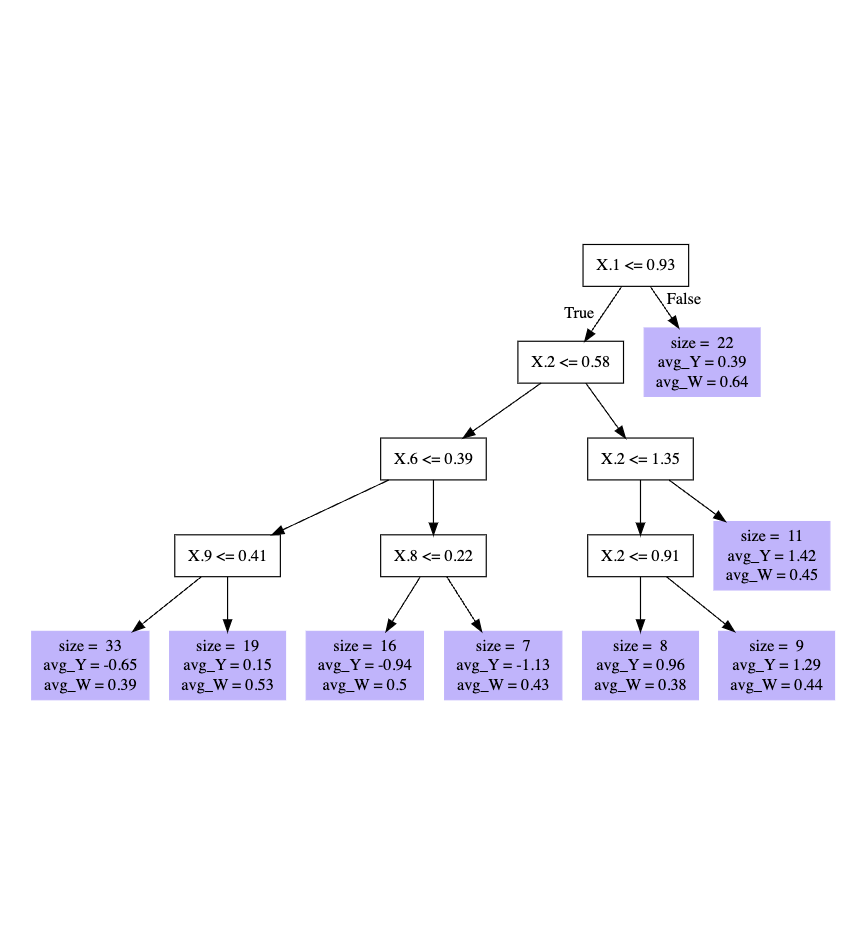
\includegraphics[width = 0.8\textwidth]{../assets/tree-plot.png}
\end{figure}
\hfill
\end{frame}


%%%%%NOTE%%%%%
\note{
\scriptsize \singlespacing

\begin{wideitemize}
\item xxxx
\end{wideitemize}

}
%-------------------------------------------------------------------------------%


\backupbegin
%-------------------------------------------------------------------------------%

\begin{frame}[allowframebreaks]{References}
    \bibliographystyle{apalike}
    \bibliography{../assets/PLSC40601}
\end{frame}
%-------------------------------------------------------------------------------%
\backupend
\end{document}
%
%-------------------------------------------------------------------------------%
%%% [[TEMPLATE]] %%%
\begin{transitionframe}
\centering

\LARGE \textcolor{white}{Statement.}

\end{transitionframe}
%-------------------------------------------------------------------------------%

%%% [[TEMPLATE]] %%%
\begin{frame}{Frametitle}

\begin{wideitemize}
\item xxx
\end{wideitemize}

\end{frame}


%%%%%NOTE%%%%%
\note{
\scriptsize \singlespacing

\begin{wideitemize}
\item xxxx
\end{wideitemize}

}

%-------------------------------------------------------------------------------%
